\chapter{Signal, Noise, and Detection in CCD Photometry}

	A CCD detector does not deliver an exact astronomical flux; rather, it accumulates discrete photoelectrons in a two-dimensional grid of pixels over a finite exposure time, and that measured count unavoidably carries statistical uncertainty. Everything that governs observational success in optical and infrared astronomy --- whether a faint object is reliably detected, how precisely its apparent magnitude can be measured, and whether an observer should integrate continuously in a single long exposure or co-add multiple short exposures --- follows from tracking that uncertainty rigorously from its underlying physical origin to the final signal-to-noise ratio ($\mathrm{SNR}$). In this chapter, we develop a complete first-principles treatment of CCD noise statistics without empirical fudge factors, deriving the Poisson nature of photon counting, formulating the master CCD signal-to-noise equation, and analyzing the three distinct observational regimes that dictate optimal observing strategy.

	\section{Fundamental Notation and Bookkeeping Conventions}

	To avoid the widespread confusion arising from reusing the letter $N$ for both total photon counts and noise amplitudes, we adopt the strict convention that every noise term is denoted by $\sigma$ (a standard deviation), while electron rates are denoted by $R$ with descriptive subscripts. The total integration time $t$ is partitioned into $N_{\rm exp}$ discrete exposures of duration $t_{\rm exp}$.

	\begin{table}[htbp]
		\centering
		\begin{tabular}{@{}l p{9.8cm} l@{}}
			\toprule
			\textbf{Symbol} & \textbf{Physical Meaning} & \textbf{Units} \\
			\midrule
			$R_{\rm src}$ & Photoelectron rate from the astronomical source integrated over the aperture & $\mathrm{e^-\,s^{-1}}$ \\
			$R_{\rm sky}$ & Sky-background photoelectron rate per pixel & $\mathrm{e^-\,s^{-1}\,pix^{-1}}$ \\
			$R_{\rm dark}$ & Thermal dark-current generation rate per pixel & $\mathrm{e^-\,s^{-1}\,pix^{-1}}$ \\
			$n_{\rm pix}$ & Number of detector pixels contained within the photometric aperture ($\propto \theta_{\rm see}^2$) & $\mathrm{pixels}$ \\
			$t_{\rm exp}$ & Exposure duration of an individual frame & $\mathrm{s}$ \\
			$N_{\rm exp}$ & Total number of individual exposures co-added & --- \\
			$t$ & Total integration time ($t = N_{\rm exp}t_{\rm exp}$) & $\mathrm{s}$ \\
			$S$ & Total source signal collected over the integration ($S = R_{\rm src}t$) & $\mathrm{e^-}$ \\
			$\sigma_{\rm RON}$ & Readout noise standard deviation per pixel per single read & $\mathrm{e^-}$ \\
			$\sigma_x$ & Standard deviation (noise contribution) associated with physical process $x$ & $\mathrm{e^-}$ \\
			$\mathrm{SNR}$ & Signal-to-noise ratio ($S/\sigma_{\rm tot}$) & --- \\
			$m, \delta m$ & Apparent magnitude and its associated photometric uncertainty & $\mathrm{mag}$ \\
			\bottomrule
		\end{tabular}
		\caption{Mathematical symbols, physical definitions, and units used throughout the CCD noise analysis.}
		\label{tab:ccd_notation}
	\end{table}

	\paragraph{Post-Quantum-Efficiency (post-QE) Convention.}
	When an incident photon strikes the silicon lattice of a CCD, it produces an electron-hole pair with probability $\eta(\lambda)$, known as the detector's \emph{quantum efficiency} (typically $\eta \sim 0.50\text{--}0.85$ in modern back-illuminated astronomical CCDs). Because $\eta$ uniformly scales all photon-driven rates, we absorb $\eta$ directly into the definitions of $R_{\rm src}$ and $R_{\rm sky}$. Counting directly in \emph{detected photoelectrons} ($\mathrm{e^-}$) simplifies the bookkeeping and ensures that every rate ($R_{\rm src}, R_{\rm sky}, R_{\rm dark}$) is defined consistently on a post-conversion basis.

	\section{Setting Up the Photometric Measurement}

	Over a total integration time $t$, the astronomical target deposits a total detected signal
	\begin{equation}
		S = R_{\rm src}\,t.
		\label{eq:ccd_signal_total}
	\end{equation}
	In practical astronomical observations, the total time $t$ is divided into $N_{\rm exp}$ separate exposures of duration $t_{\rm exp}$ each:
	\begin{equation}
		t = N_{\rm exp}\,t_{\rm exp}, \qquad S = R_{\rm src}\,N_{\rm exp}\,t_{\rm exp}.
		\label{eq:ccd_signal_partition}
	\end{equation}
	This distinction between the total accumulated time $t$ and its subdivision into $N_{\rm exp}$ sub-exposures is crucial: while Poisson photon accumulation depends only on total time $t$, readout noise is incurred afresh on every single readout and scales directly with $N_{\rm exp}$.

	\section{Photometric Precision, Magnitude Uncertainty, and Detection Significance}

	The noise $\sigma_{\rm tot}$ represents the $1\sigma$ standard deviation of the measured source signal $S$, so that the measurement is reported as $S \pm \sigma_{\rm tot}$. The signal-to-noise ratio is defined as
	\begin{keyresult}
		\begin{equation}
			\mathrm{SNR} \equiv \frac{S}{\sigma_{\rm tot}}.
			\label{eq:snr_def}
		\end{equation}
	\end{keyresult}
	The reciprocal $1/\mathrm{SNR} = \sigma_{\rm tot}/S$ represents the fractional uncertainty of the flux measurement. Table~\ref{tab:snr_benchmarks} summarizes the observational meaning of typical $\mathrm{SNR}$ values.

	\begin{table}[htbp]
		\centering
		\begin{tabular}{@{}l l p{8.5cm}@{}}
			\toprule
			\textbf{SNR} & \textbf{Fractional Error $1/\mathrm{SNR}$} & \textbf{Observational Regime and Practical Meaning} \\
			\midrule
			2--3 & 33--50\% & Object barely detected; high risk of false alarm in blind searches. \\
			5 & 20\% & Robust detection threshold ($5\sigma$ standard); true physical source. \\
			10 & 10\% & Standard photometric measurement ($\sim 0.1\,\mathrm{mag}$ precision). \\
			100 & 1\% & Precision astrophysics (exoplanet transits, stellar variability, $\sim 0.01\,\mathrm{mag}$). \\
			\bottomrule
		\end{tabular}
		\caption{Astronomical signal-to-noise ratio benchmarks and their observational interpretation.}
		\label{tab:snr_benchmarks}
	\end{table}

	\subsection{Error Propagation from Electron Counts to Magnitudes}

	Astronomical brightness is reported on Pogson's logarithmic magnitude scale, $m = -2.5\log_{10}(S) + C_0$, where $C_0$ is a photometric zero-point constant independent of $S$. If the true signal $S$ is perturbed by the $1\sigma$ uncertainty $\sigma_{\rm tot}$, the corresponding magnitude shift is
	\begin{equation}
		\delta m = 2.5\log_{10}\!\left(\frac{S + \sigma_{\rm tot}}{S}\right) = 2.5\log_{10}\!\left(1 + \frac{\sigma_{\rm tot}}{S}\right) = 2.5\log_{10}\!\left(1 + \frac{1}{\mathrm{SNR}}\right).
		\label{eq:exact_mag_error}
	\end{equation}
	For high signal-to-noise ratios ($\mathrm{SNR} \gg 1$), we use the Taylor expansion $\ln(1+x) \approx x$ with $\log_{10}(1+x) = \frac{\ln(1+x)}{\ln 10} \approx \frac{x}{\ln 10}$:
	\begin{keyresult}
		\begin{equation}
			\delta m \approx \frac{2.5}{\ln 10}\cdot\frac{\sigma_{\rm tot}}{S} = \frac{1.0857}{\mathrm{SNR}}.
			\label{eq:linear_mag_error}
		\end{equation}
	\end{keyresult}

	\begin{tcolorbox}[notebox, title=CHECKED NUMERICALLY]
		The exact logarithmic expression (Eq.~\eqref{eq:exact_mag_error}) and the first-order linear approximation (Eq.~\eqref{eq:linear_mag_error}) show exceptional agreement for $\mathrm{SNR} \ge 10$, where the relative difference is less than $5\%$. However, for low signal-to-noise ratios ($\mathrm{SNR} \le 3$), the linear approximation underestimates the true asymmetric uncertainty, requiring the exact logarithmic formulation shown in Figure~\ref{fig:dmag_comparison}.
	\end{tcolorbox}

	\begin{figure}[htbp]
		\centering
		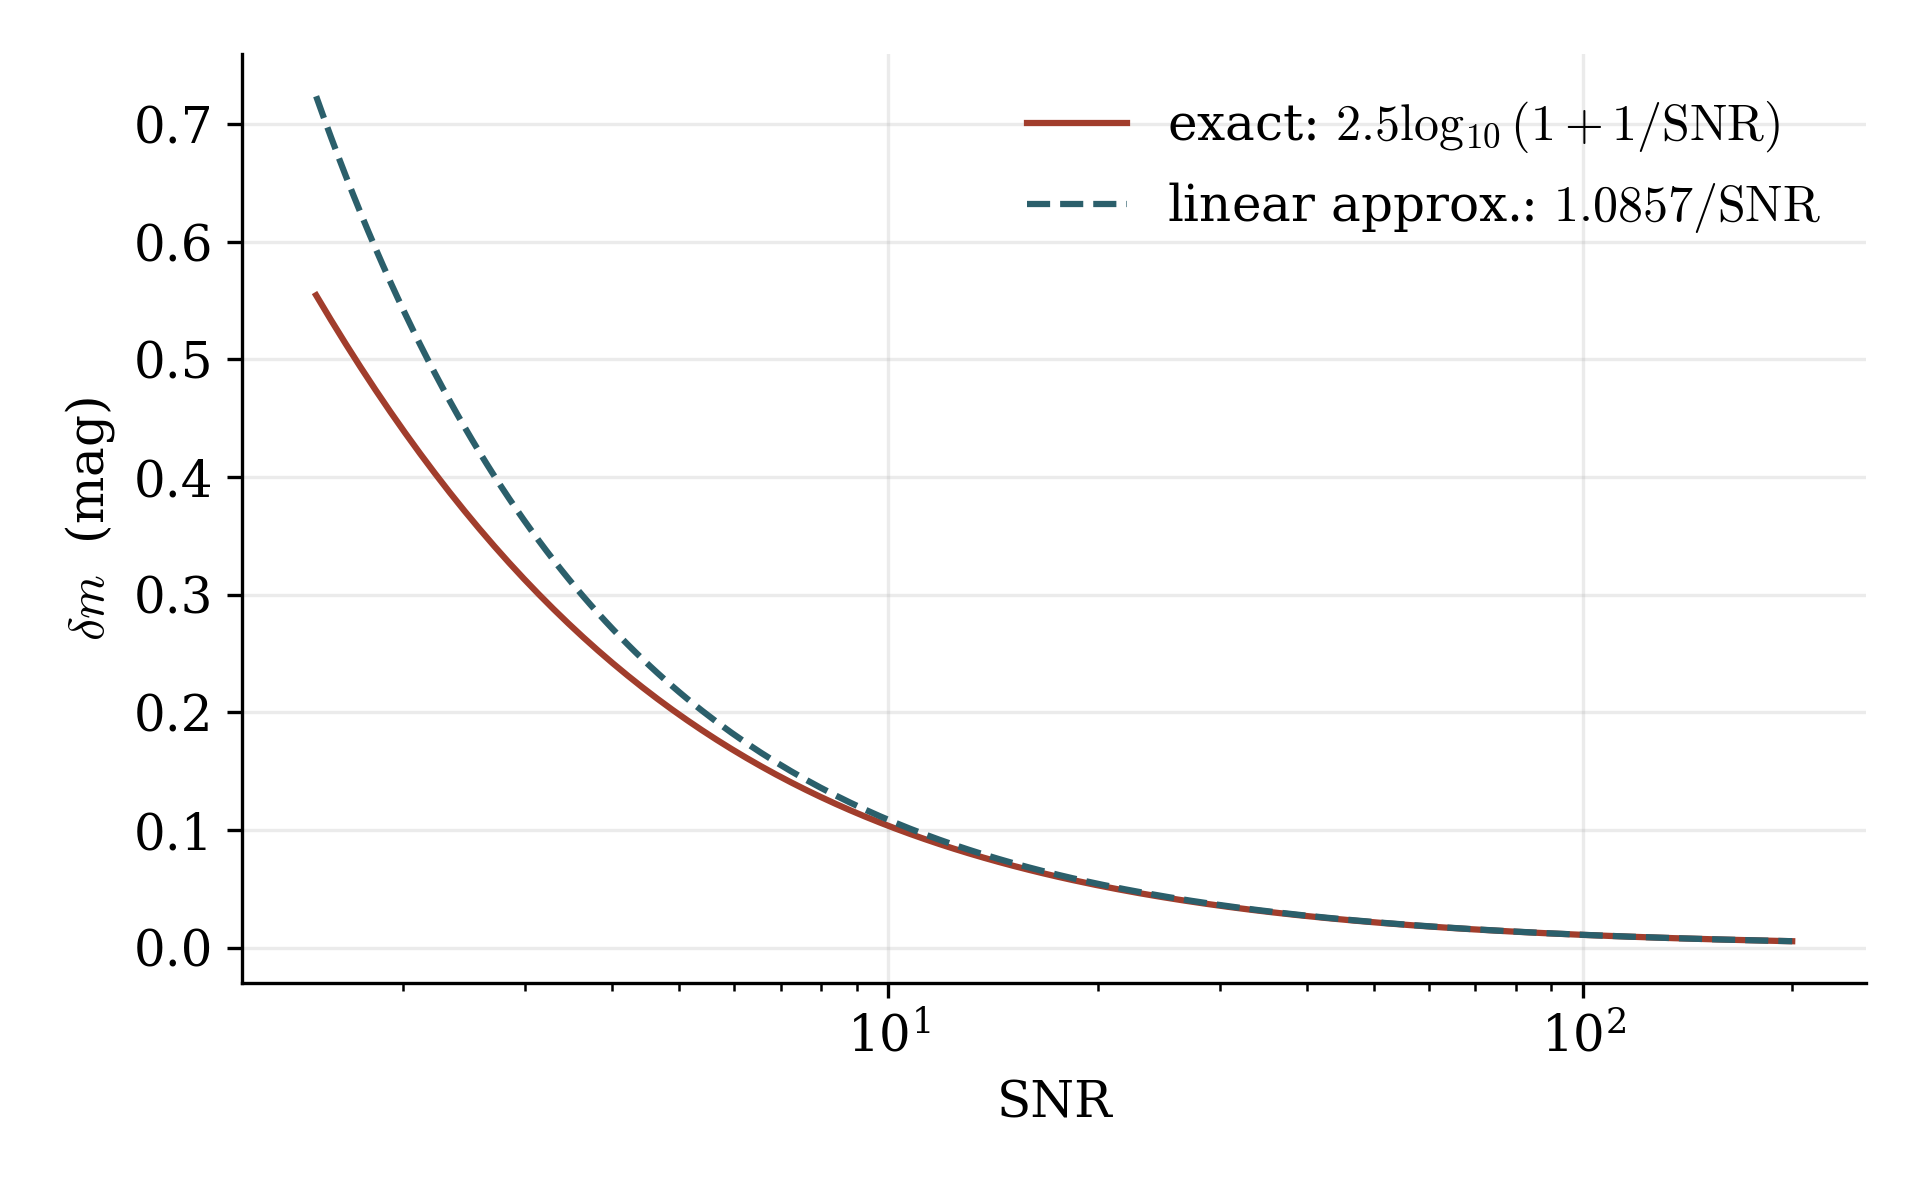
\includegraphics[width=0.72\textwidth]{figs/fig3_dmag.png}
		\caption{Exact photometric magnitude error $\delta m$ compared against the first-order approximation $\delta m \approx 1.0857/\mathrm{SNR}$ as a function of $\mathrm{SNR}$. The curves converge above $\mathrm{SNR}\sim 10$ and diverge significantly below $\mathrm{SNR}\sim 5$.}
		\label{fig:dmag_comparison}
	\end{figure}

	\subsection{Detection Significance and the False-Alarm Probability}

	At the low-SNR threshold ($\mathrm{SNR} = 2\text{--}5$), the central question is whether an observed signal corresponds to a genuine astrophysical source or merely an extreme statistical fluctuation of the background.

	\paragraph{Gaussian Noise Assumption via the Central Limit Theorem.}
	Because the total detected electron count is the sum of many independent Poisson-distributed quantum events and amplifier readouts across multiple pixels, the Central Limit Theorem guarantees that the distribution of total noise $\sigma_{\rm tot}$ is exceedingly well approximated by a Gaussian (normal) distribution $\mathcal{N}(0, \sigma_{\rm tot}^2)$. This justifies expressing detection thresholds in units of standard deviations ($k\sigma$).

	In the null hypothesis (where no astronomical source is present, $S=0$), the probability that pure background noise fluctuates upward by at least $k\sigma_{\rm tot}$ is given by the complementary standard normal cumulative distribution function (Gaussian upper tail):
	\begin{keyresult}
		\begin{equation}
			P(k) = \int_{k}^{\infty} \frac{1}{\sqrt{2\pi}} e^{-x^2/2}\,dx = 1 - \Phi(k).
			\label{eq:false_alarm_single}
		\end{equation}
	\end{keyresult}

	\begin{tcolorbox}[notebox, title=NUMERICAL EVALUATION OF FALSE-ALARM PROBABILITIES]
		Evaluating the Gaussian tail integral numerically:
		\begin{itemize}
			\item $k = 2\sigma$: $P(2) = 2.28 \times 10^{-2}$ ($\sim 1 \text{ in } 44$)
			\item $k = 3\sigma$: $P(3) = 1.35 \times 10^{-3}$ ($\sim 1 \text{ in } 741$)
			\item $k = 5\sigma$: $P(5) = 2.87 \times 10^{-7}$ ($\sim 1 \text{ in } 3.48 \text{ million}$)
			\item $k = 10\sigma$: $P(10) = 7.62 \times 10^{-24}$ ($\sim \text{physically impossible by pure chance}$)
		\end{itemize}
		The steep exponential decline of false-alarm probability with increasing significance is plotted in Figure~\ref{fig:gaussian_tail_prob}.
	\end{tcolorbox}

	\begin{figure}[htbp]
		\centering
		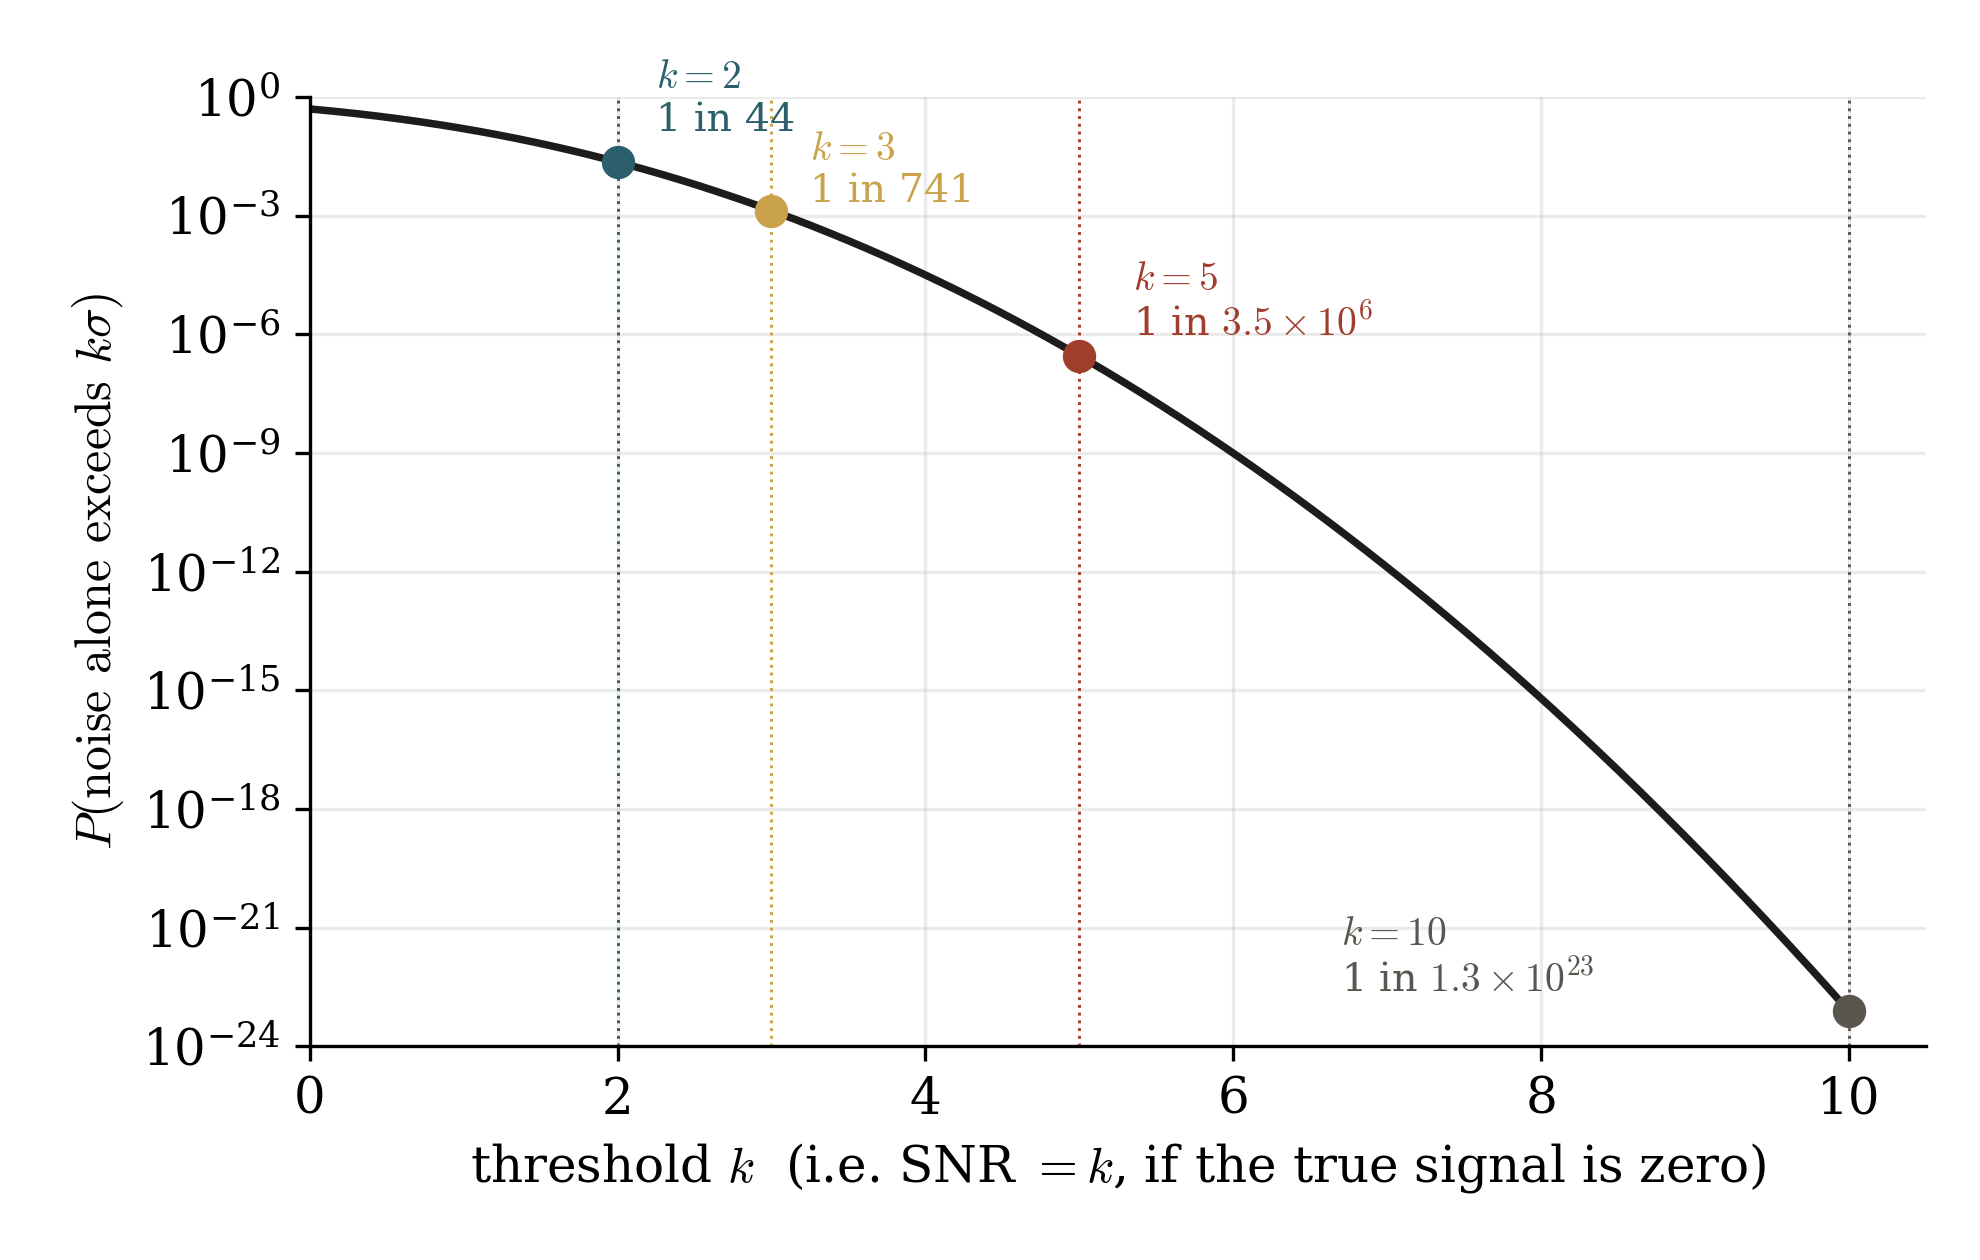
\includegraphics[width=0.72\textwidth]{figs/fig_gaussian_tail.png}
		\caption{Single-trial false-alarm probability $P(k)$ that zero-mean Gaussian background noise generates an apparent excess exceeding $k\sigma$, plotted on a logarithmic scale.}
		\label{fig:gaussian_tail_prob}
	\end{figure}

	\subsection{The Look-Elsewhere Effect and Multi-Pixel Detection Thresholds}

	The single-trial probability $P(k)$ applies when evaluating a pre-specified location (e.g., measuring the flux of a known target star). However, in wide-field blind searches (transient detection, asteroid searches, survey discovery), one tests $n_{\rm trial}$ independent resolution elements simultaneously.

	\begin{tcolorbox}[flagbox, title=THE CATCH: FALSE ALARMS SCALE WITH SEARCH VOLUME]
		If an image contains $n_{\rm trial}$ independent apertures or resolution elements, the probability that \emph{at least one} pure-noise fluctuation exceeds $k\sigma$ is bounded by the union bound:
		\begin{equation}
			P_{\rm any}(k) \approx n_{\rm trial}\,P(k).
			\label{eq:union_bound}
		\end{equation}
		For a modern $4000 \times 4000$ CCD detector ($n_{\rm trial} \approx 1.6 \times 10^7$ pixels):
		\begin{itemize}
			\item At $k=3\sigma$: Expected noise false positives $= (1.6 \times 10^7) \times (1.35 \times 10^{-3}) \approx 2.2 \times 10^4$ spurious detections! The survey is hopelessly swamped by artifacts.
			\item At $k=5\sigma$: Expected noise false positives $= (1.6 \times 10^7) \times (2.87 \times 10^{-7}) \approx 4.6$ false detections across the entire mosaic.
			\item At $k \ge 5.5\sigma$: Expected noise false positives $< 0.3$, guaranteeing that any candidate is almost certainly real.
		\end{itemize}
		This explains why large-scale astronomical surveys universally enforce a $5\sigma$ threshold for discovery claims.
	\end{tcolorbox}

	\section{Physical Origins of Noise in CCD Measurements}

	The total uncertainty $\sigma_{\rm tot}$ is not a monolithic quantity. It is the quadrature sum of four physically distinct processes: photon shot noise from the source, shot noise from the sky background, shot noise from thermal dark current, and readout noise from on-chip amplifiers.

	\subsection{First-Principles Derivation of Photon Shot Noise}

	Even if an astronomical source emits at a perfectly steady mean luminosity, the number of photoelectrons collected in consecutive equal intervals fluctuates. This fundamental variance arises because electromagnetic radiation is quantized: photons arrive as discrete, independent packets.

	\paragraph{Derivation from the Binomial Distribution.}
	Let photons arrive at a constant average rate $\lambda$ (photons per second). Divide the exposure time $t$ into $N$ infinitesimal time bins of duration $\Delta t = t/N$. In each subinterval, the probability of detecting a single photon is $p = \lambda\Delta t = \mu/N$ (where $\mu = \lambda t$ is the expected total count), while the probability of multiple arrivals in the same subinterval approaches zero as $N \to \infty$.

	Because the arrival in each subinterval is an independent Bernoulli trial, the probability of obtaining exactly $n$ arrivals in $N$ subintervals follows the Binomial distribution:
	\begin{equation}
		P(n) = \binom{N}{n} p^n (1-p)^{N-n} = \frac{N!}{n!(N-n)!}\left(\frac{\mu}{N}\right)^n \left(1 - \frac{\mu}{N}\right)^{N-n}.
	\end{equation}
	Taking the continuous limit $N \to \infty$ with $\mu$ held fixed, using $\frac{N!}{(N-n)!N^n} \to 1$ and $(1 - \mu/N)^N \to e^{-\mu}$, we recover the \emph{Poisson distribution}:
	\begin{keyresult}
		\begin{equation}
			P(n;\mu) = \frac{\mu^n e^{-\mu}}{n!}.
			\label{eq:poisson_dist}
		\end{equation}
	\end{keyresult}

	\paragraph{Derivation of Mean and Variance.}
	The expectation value of $n$ is:
	\begin{equation}
		\langle n \rangle = \sum_{n=0}^{\infty} n\,\frac{\mu^n e^{-\mu}}{n!} = \mu e^{-\mu}\sum_{n=1}^{\infty} \frac{\mu^{n-1}}{(n-1)!} = \mu e^{-\mu} e^{\mu} = \mu.
		\label{eq:poisson_mean}
	\end{equation}
	Evaluating the second factorial moment $\langle n(n-1)\rangle$:
	\begin{equation}
		\langle n(n-1) \rangle = \sum_{n=0}^{\infty} n(n-1)\,\frac{\mu^n e^{-\mu}}{n!} = \mu^2 e^{-\mu}\sum_{n=2}^{\infty}\frac{\mu^{n-2}}{(n-2)!} = \mu^2 e^{-\mu} e^{\mu} = \mu^2.
	\end{equation}
	Since $\langle n^2 \rangle = \langle n(n-1)\rangle + \langle n\rangle = \mu^2 + \mu$, the variance is:
	\begin{equation}
		\mathrm{Var}(n) = \langle n^2 \rangle - \langle n\rangle^2 = (\mu^2 + \mu) - \mu^2 = \mu.
		\label{eq:poisson_var}
	\end{equation}
	The standard deviation (shot noise) is therefore:
	\begin{keyresult}
		\begin{equation}
			\sigma = \sqrt{\mathrm{Var}(n)} = \sqrt{\mu}.
			\label{eq:shot_noise_sigma}
		\end{equation}
	\end{keyresult}

	\begin{tcolorbox}[notebox, title=CHECKED NUMERICALLY]
		For $\mu=10$, summing Eq.~\eqref{eq:poisson_dist} directly (truncated at $n=200$) gives $\sum_n P(n)=1.0000$, $\langle n\rangle = 10.000$, and $\mathrm{Var}(n)=10.000$ --- confirming the analytical results.
	\end{tcolorbox}

	\begin{figure}[htbp]
		\centering
		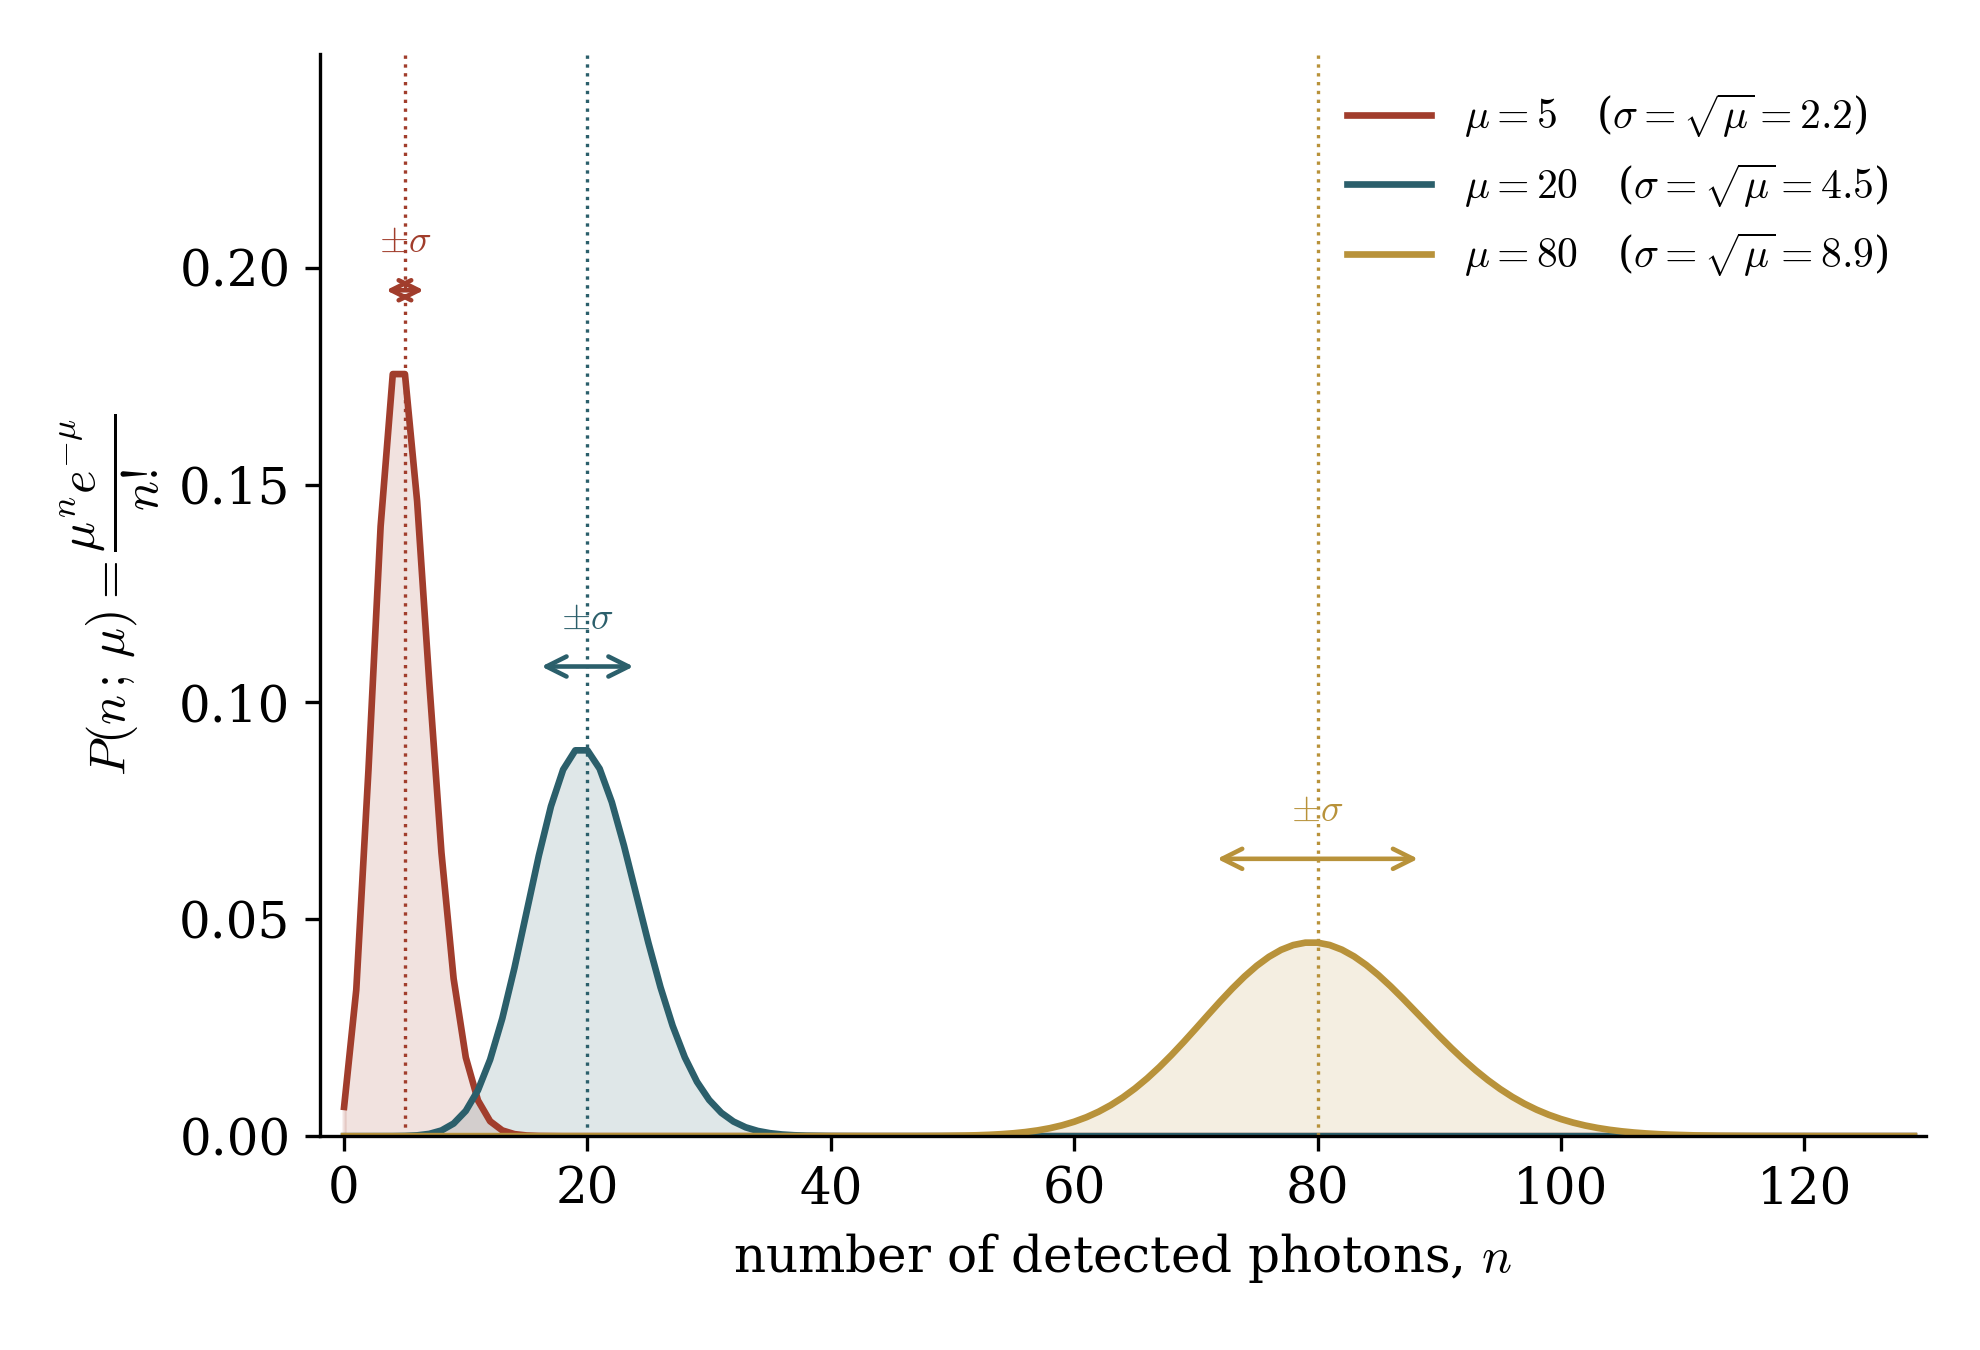
\includegraphics[width=0.82\textwidth]{figs/fig0_poisson.png}
		\caption{The Poisson probability distribution $P(n;\mu)$ for mean counts $\mu = 10, 50, 250$. While the absolute standard deviation $\sigma = \sqrt{\mu}$ grows with brightness, the relative fractional noise $\sigma/\mu = 1/\sqrt{\mu}$ contracts, leading directly to the $\mathrm{SNR} \propto \sqrt{\mu}$ scaling of photon-limited measurements.}
		\label{fig:poisson_distributions}
	\end{figure}

	\subsection{The Three Counting Shot-Noise Contributions}

	Applying Eq.~\eqref{eq:shot_noise_sigma} to each independent physical source of photoelectrons:

	\begin{enumerate}
		\item \textbf{Object Shot Noise:} The astronomical source delivers $S = R_{\rm src}t$ photoelectrons inside the aperture, giving:
		\begin{equation}
			\sigma_{\rm src} = \sqrt{S} = \sqrt{R_{\rm src}\,t}.
			\label{eq:sigma_src}
		\end{equation}

		\item \textbf{Sky Background Shot Noise:} The sky background emits photons uniformly across the focal plane at rate $R_{\rm sky}$ per pixel. Over an aperture of $n_{\rm pix}$ pixels during exposure $t$, the accumulated sky electrons are $n_{\rm pix}R_{\rm sky}t$. Although the mean sky level is subtracted during data reduction, its Poisson fluctuation remains:
		\begin{equation}
			\sigma_{\rm sky} = \sqrt{n_{\rm pix}\,R_{\rm sky}\,t}.
			\label{eq:sigma_sky}
		\end{equation}
		Because the required photometric aperture area scales with seeing disk size ($n_{\rm pix} \propto \theta_{\rm see}^2$), superior seeing directly reduces sky noise.

		\item \textbf{Dark Current Shot Noise:} Thermal vibrations in the silicon lattice spontaneously generate electron-hole pairs at rate $R_{\rm dark}$ per pixel. These accumulate over $n_{\rm pix}$ pixels and duration $t$:
		\begin{equation}
			\sigma_{\rm dark} = \sqrt{n_{\rm pix}\,R_{\rm dark}\,t}.
			\label{eq:sigma_dark}
		\end{equation}
	\end{enumerate}

	\begin{tcolorbox}[flagbox, title=UNITS CAUTION: DARK CURRENT CONVERSIONS]
		Manufacturers and detector manuals frequently quote dark current in units of $\mathrm{e^-\,pixel^{-1}\,hr^{-1}}$. When inserting $R_{\rm dark}$ into Eq.~\eqref{eq:sigma_dark} with exposure time $t$ in seconds, $R_{\rm dark}$ must be converted to $\mathrm{e^-\,s^{-1}\,pix^{-1}}$:
		\[
		R_{\rm dark}\,[\mathrm{e^-\,s^{-1}\,pix^{-1}}] = \frac{R_{\rm dark}\,[\mathrm{e^-\,hr^{-1}\,pix^{-1}}]}{3600\,\mathrm{s/hr}}.
		\]
		Throughout these notes, all rates ($R_{\rm src}, R_{\rm sky}, R_{\rm dark}$) are strictly in $\mathrm{e^-\,s^{-1}}$.
	\end{tcolorbox}

	\subsection{Readout Noise: The Additive Amplifier Penalty}

	Unlike the three counting processes above, readout noise is \emph{not} a shot noise. It arises from thermal (Johnson-Nyquist) and flicker ($1/f$) electronic noise in the output field-effect transistor (FET) and analog-to-digital converter (ADC) during charge-to-voltage conversion.

	Readout noise adds a constant Gaussian uncertainty $\sigma_{\rm RON}$ (in electrons RMS) to each pixel per readout, independent of exposure time. For $n_{\rm pix}$ pixels read out in each of $N_{\rm exp}$ independent exposures:
	\begin{keyresult}
		\begin{equation}
			\sigma_{\rm read} = \sqrt{n_{\rm pix}\,N_{\rm exp}}\;\sigma_{\rm RON}.
			\label{eq:sigma_read}
		\end{equation}
	\end{keyresult}
	Note the fundamental structural difference: $\sigma_{\rm read}^2 \propto N_{\rm exp}$ rather than $\propto t$. Splitting an exposure of duration $t$ into $N_{\rm exp}$ shorter exposures incurs the read noise penalty $N_{\rm exp}$ times in variance.

	\section{The Master Signal-to-Noise Ratio Equation}

	\begin{tcolorbox}[notebox, title=FIRST-PRINCIPLES DERIVATION: WHY VARIANCES ADD FOR INDEPENDENT NOISE SOURCES]
		Let $X$ and $Y$ be two random variables representing independent physical noise processes with expected values $\mu_X = \mathbb{E}[X]$, $\mu_Y = \mathbb{E}[Y]$ and variances $\sigma_X^2 = \mathrm{Var}(X)$, $\sigma_Y^2 = \mathrm{Var}(Y)$.

		The variance of their sum $Z = X + Y$ is defined by:
		\begin{equation}
			\mathrm{Var}(X + Y) = \mathbb{E}\left[\big((X + Y) - \mathbb{E}[X + Y]\big)^2\right] = \mathbb{E}\left[\big((X - \mu_X) + (Y - \mu_Y)\big)^2\right].
		\end{equation}
		Expanding the algebraic square inside the expectation:
		\begin{equation}
			\big((X - \mu_X) + (Y - \mu_Y)\big)^2 = (X - \mu_X)^2 + (Y - \mu_Y)^2 + 2(X - \mu_X)(Y - \mu_Y).
		\end{equation}
		Applying the linearity of the mathematical expectation operator $\mathbb{E}[\,\cdot\,]$:
		\begin{align}
			\mathrm{Var}(X + Y) &= \mathbb{E}\left[(X - \mu_X)^2\right] + \mathbb{E}\left[(Y - \mu_Y)^2\right] + 2\,\mathbb{E}\left[(X - \mu_X)(Y - \mu_Y)\right] \notag \\
			&= \mathrm{Var}(X) + \mathrm{Var}(Y) + 2\,\mathrm{Cov}(X, Y).
		\end{align}
		Because the physical mechanisms generating astronomical source photons, sky background photons, thermal dark current, and amplifier readout noise are statistically \emph{independent}, their joint probability density factorizes: $p(x, y) = p_X(x)\,p_Y(y)$. The covariance therefore vanishes identically:
		\begin{equation}
			\mathrm{Cov}(X, Y) = \mathbb{E}[(X - \mu_X)]\,\mathbb{E}[(Y - \mu_Y)] = 0 \cdot 0 = 0.
		\end{equation}
		By mathematical induction, for $N$ mutually independent noise contributions $X_1, X_2, \dots, X_N$:
		\begin{equation}
			\mathrm{Var}\left(\sum_{i=1}^N X_i\right) = \sum_{i=1}^N \mathrm{Var}(X_i) \quad\Longrightarrow\quad \sigma_{\rm tot}^2 = \sum_{i=1}^N \sigma_i^2 \quad\Longleftrightarrow\quad \sigma_{\rm tot} = \sqrt{\sum_{i=1}^N \sigma_i^2}.
		\end{equation}
		This rigorous result proves why independent noise contributions must be added in quadrature, establishing the fundamental basis of the CCD noise budget.
	\end{tcolorbox}

	Because the four noise sources arise from statistically independent physical mechanisms, their variances add in quadrature:
	\begin{equation}
		\sigma_{\rm tot}^2 = \sigma_{\rm src}^2 + \sigma_{\rm sky}^2 + \sigma_{\rm dark}^2 + \sigma_{\rm read}^2.
		\label{eq:variance_addition}
	\end{equation}
	Substituting the derived expressions into Eq.~\eqref{eq:snr_def} yields the \textbf{Master CCD Signal-to-Noise Equation}:

	\begin{tcolorbox}[enhanced, colback=white, colframe=ink, boxrule=0.9pt, arc=0pt, left=14pt, right=14pt, top=10pt, bottom=10pt]
		\begin{equation}
			\mathrm{SNR} = \frac{R_{\rm src}\,t}{\sqrt{R_{\rm src}\,t \;+\; n_{\rm pix}R_{\rm sky}\,t \;+\; n_{\rm pix}R_{\rm dark}\,t \;+\; n_{\rm pix}N_{\rm exp}\,\sigma_{\rm RON}^2}}
			\label{eq:master_ccd_snr}
		\end{equation}
	\end{tcolorbox}
	where $t = N_{\rm exp}t_{\rm exp}$. This single equation governs all exposure time calculators (ETCs) in observational astronomy.

	\begin{figure}[htbp]
		\centering
		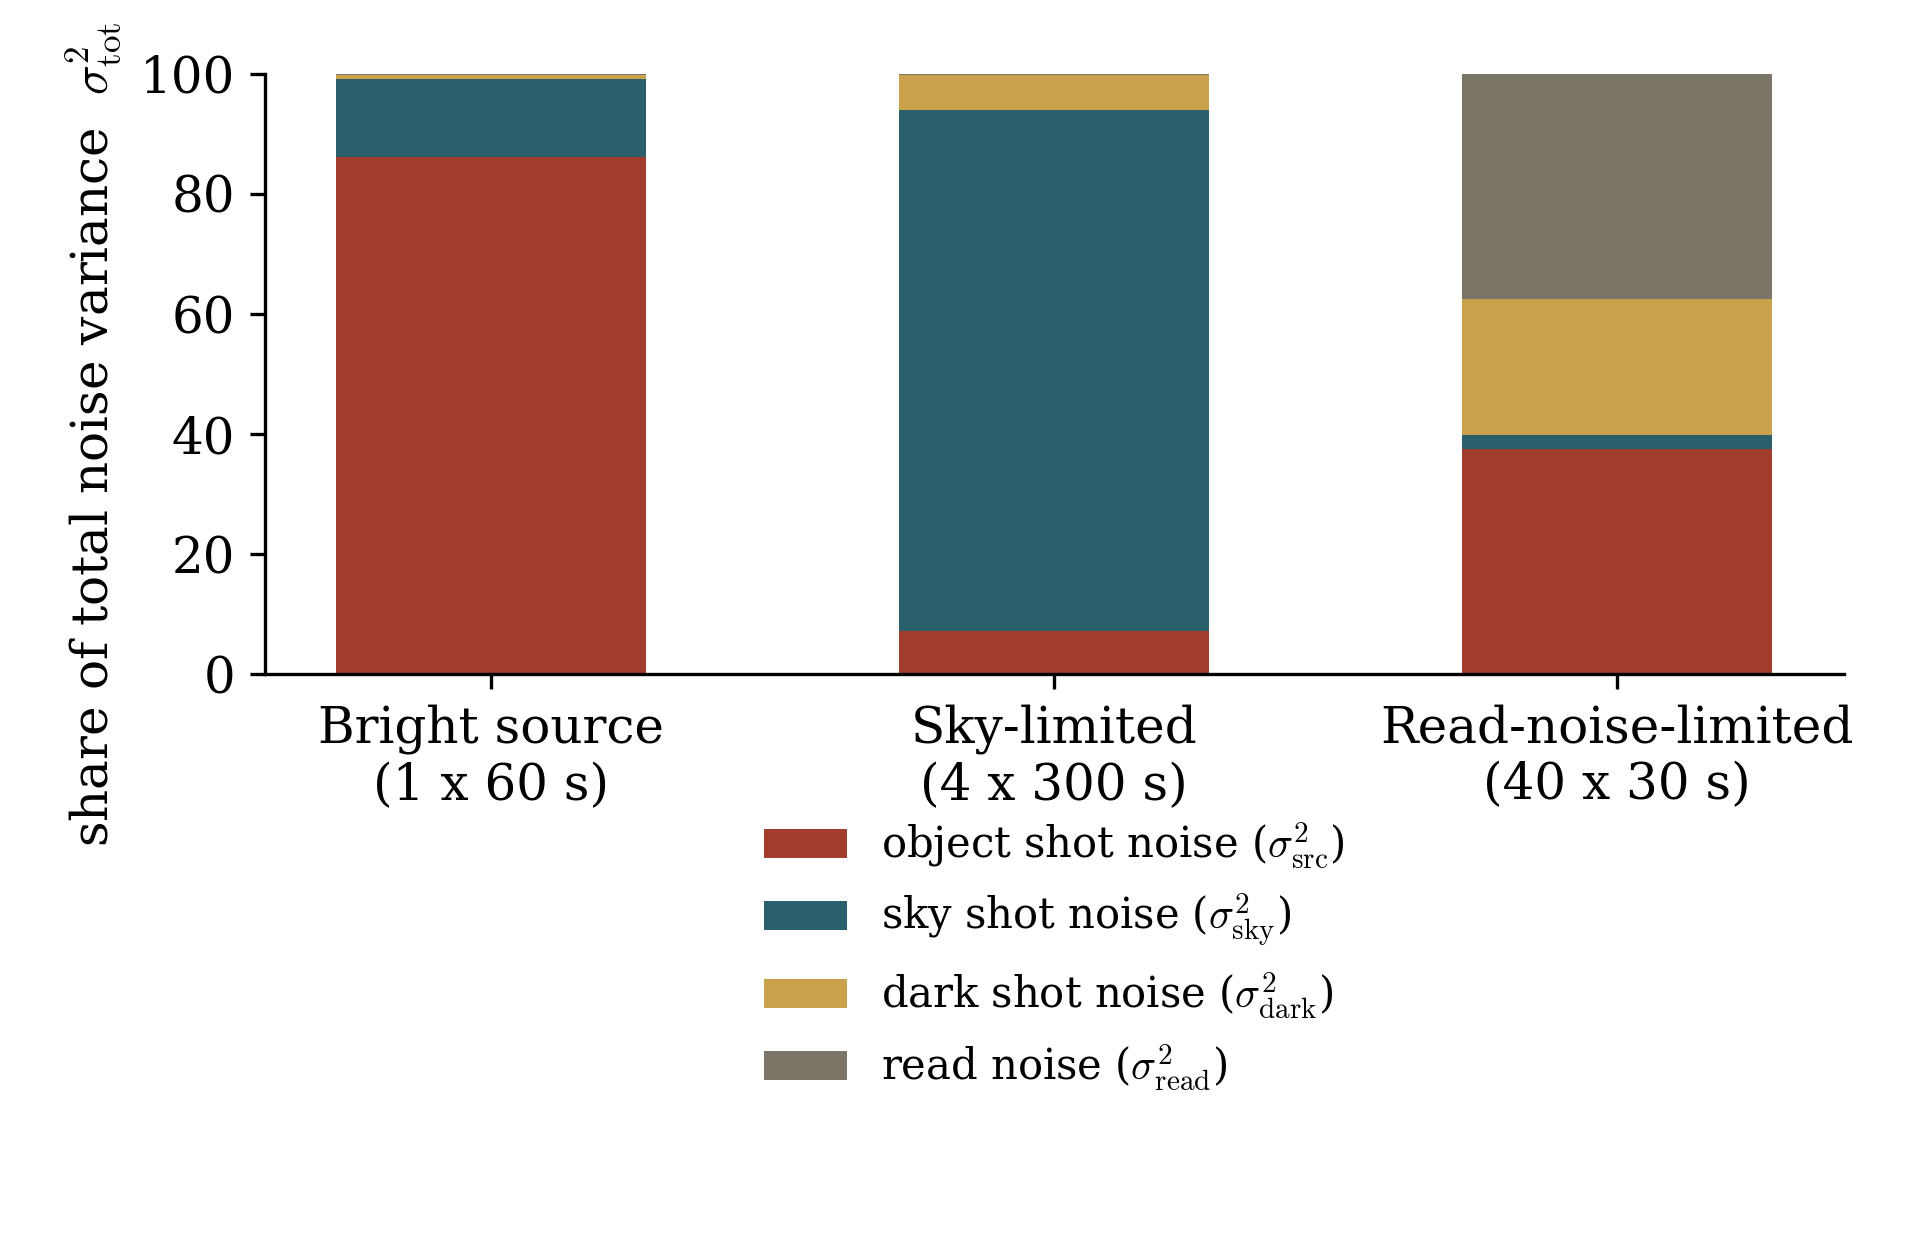
\includegraphics[width=0.85\textwidth]{figs/fig1_budget.png}
		\caption{Relative variance budget ($\sigma_i^2/\sigma_{\rm tot}^2 \times 100\%$) across three characteristic observational scenarios. Identifying which variance component dominates dictates the optimal observational strategy.}
		\label{fig:noise_budget}
	\end{figure}

	\section{The Three Observational Regimes and Exposure Planning Strategies}

	Depending on target flux, background brightness, and detector characteristics, the master equation simplifies into three distinct physical regimes.

	\subsection{Regime 1: Bright Source (Photon Shot-Noise Limited)}
	When observing a bright star, the source count rate dominates over sky, dark current, and read noise ($R_{\rm src}t \gg n_{\rm pix}(R_{\rm sky} + R_{\rm dark})t + n_{\rm pix}N_{\rm exp}\sigma_{\rm RON}^2$):
	\begin{keyresult}
		\begin{equation}
			\mathrm{SNR} \approx \frac{R_{\rm src}t}{\sqrt{R_{\rm src}t}} = \sqrt{R_{\rm src}t} \propto \sqrt{t}.
			\label{eq:regime_bright}
		\end{equation}
	\end{keyresult}
	\paragraph{Observational Strategy.} The limitation in this regime is never achieving adequate $\mathrm{SNR}$, but avoiding detector saturation (full-well capacity, typically $\sim 10^5\,\mathrm{e^-/pixel}$) and non-linear response. Observers should shorten $t_{\rm exp}$ or defocus the telescope (spread light over more pixels) to prevent saturation while accumulating the desired total photon count.

	\subsection{Regime 2: Sky-Background Limited}
	For faint targets observed in broadband optical filters, the night sky background is much brighter than the source ($n_{\rm pix}R_{\rm sky}t \gg R_{\rm src}t, n_{\rm pix}R_{\rm dark}t, n_{\rm pix}N_{\rm exp}\sigma_{\rm RON}^2$):
	\begin{keyresult}
		\begin{equation}
			\mathrm{SNR} \approx \frac{R_{\rm src}t}{\sqrt{n_{\rm pix}R_{\rm sky}t}} = \frac{R_{\rm src}\sqrt{t}}{\sqrt{n_{\rm pix}R_{\rm sky}}} \propto \frac{\sqrt{t}}{\sqrt{n_{\rm pix}}}.
			\label{eq:regime_sky}
		\end{equation}
	\end{keyresult}
	\paragraph{Observational Strategies.}
	\begin{itemize}
		\item \textbf{Seeing is paramount:} Because $n_{\rm pix} \propto \theta_{\rm see}^2$, the signal-to-noise ratio scales as $\mathrm{SNR} \propto 1/\theta_{\rm see}$. Improving seeing from $1.2''$ to $0.6''$ doubles the $\mathrm{SNR}$ (equivalent to a factor of 4 reduction in required telescope integration time).
		\item \textbf{Sub-exposure splitting is free:} In this regime, $\mathrm{SNR}$ depends strictly on total integration time $t$, not on the number of frames $N_{\rm exp}$. Splitting a $3000\,\mathrm{s}$ integration into ten $300\,\mathrm{s}$ frames incurs negligible read-noise penalty while enabling robust cosmic-ray rejection, dithering to remove bad pixels, and dynamic range preservation.
	\end{itemize}

	\subsection{Regime 3: Readout-Noise Limited}
	When observing faint objects under low background levels (narrow-band filters, high-resolution spectroscopy, or very short exposures), the readout noise dominates ($n_{\rm pix}N_{\rm exp}\sigma_{\rm RON}^2 \gg (R_{\rm src} + n_{\rm pix}R_{\rm sky} + n_{\rm pix}R_{\rm dark})t$):
	\begin{keyresult}
		\begin{equation}
			\mathrm{SNR} \approx \frac{R_{\rm src}t}{\sqrt{n_{\rm pix}N_{\rm exp}}\,\sigma_{\rm RON}} \propto \frac{1}{\sqrt{n_{\rm pix}}}\cdot\frac{1}{\sqrt{N_{\rm exp}}}.
			\label{eq:regime_read}
		\end{equation}
	\end{keyresult}
	\paragraph{Observational Strategies.}
	\begin{itemize}
		\item \textbf{On-Chip Pixel Binning:} Binning pixels on-chip (e.g., $2\times 2$) combines charges in the shift registers before readout, reducing the effective $n_{\rm pix}$ by a factor of 4 and boosting $\mathrm{SNR}$ by $\sqrt{4} = 2$ without increasing read noise. Binning should be applied up to the Nyquist limit ($\sim 2\text{--}3$ binned pixels across the seeing FWHM or resolution element).
		\item \textbf{Maximize Individual Exposure Duration:} Because $\mathrm{SNR} \propto 1/\sqrt{N_{\rm exp}}$ at fixed total time $t$, one should make $t_{\rm exp}$ as long as possible (minimizing $N_{\rm exp}$). The maximum safe exposure length is typically limited by cosmic-ray hit density ($\sim 30\text{--}45\,\mathrm{min}$ for ground-based CCDs).
	\end{itemize}

	\begin{figure}[htbp]
		\centering
		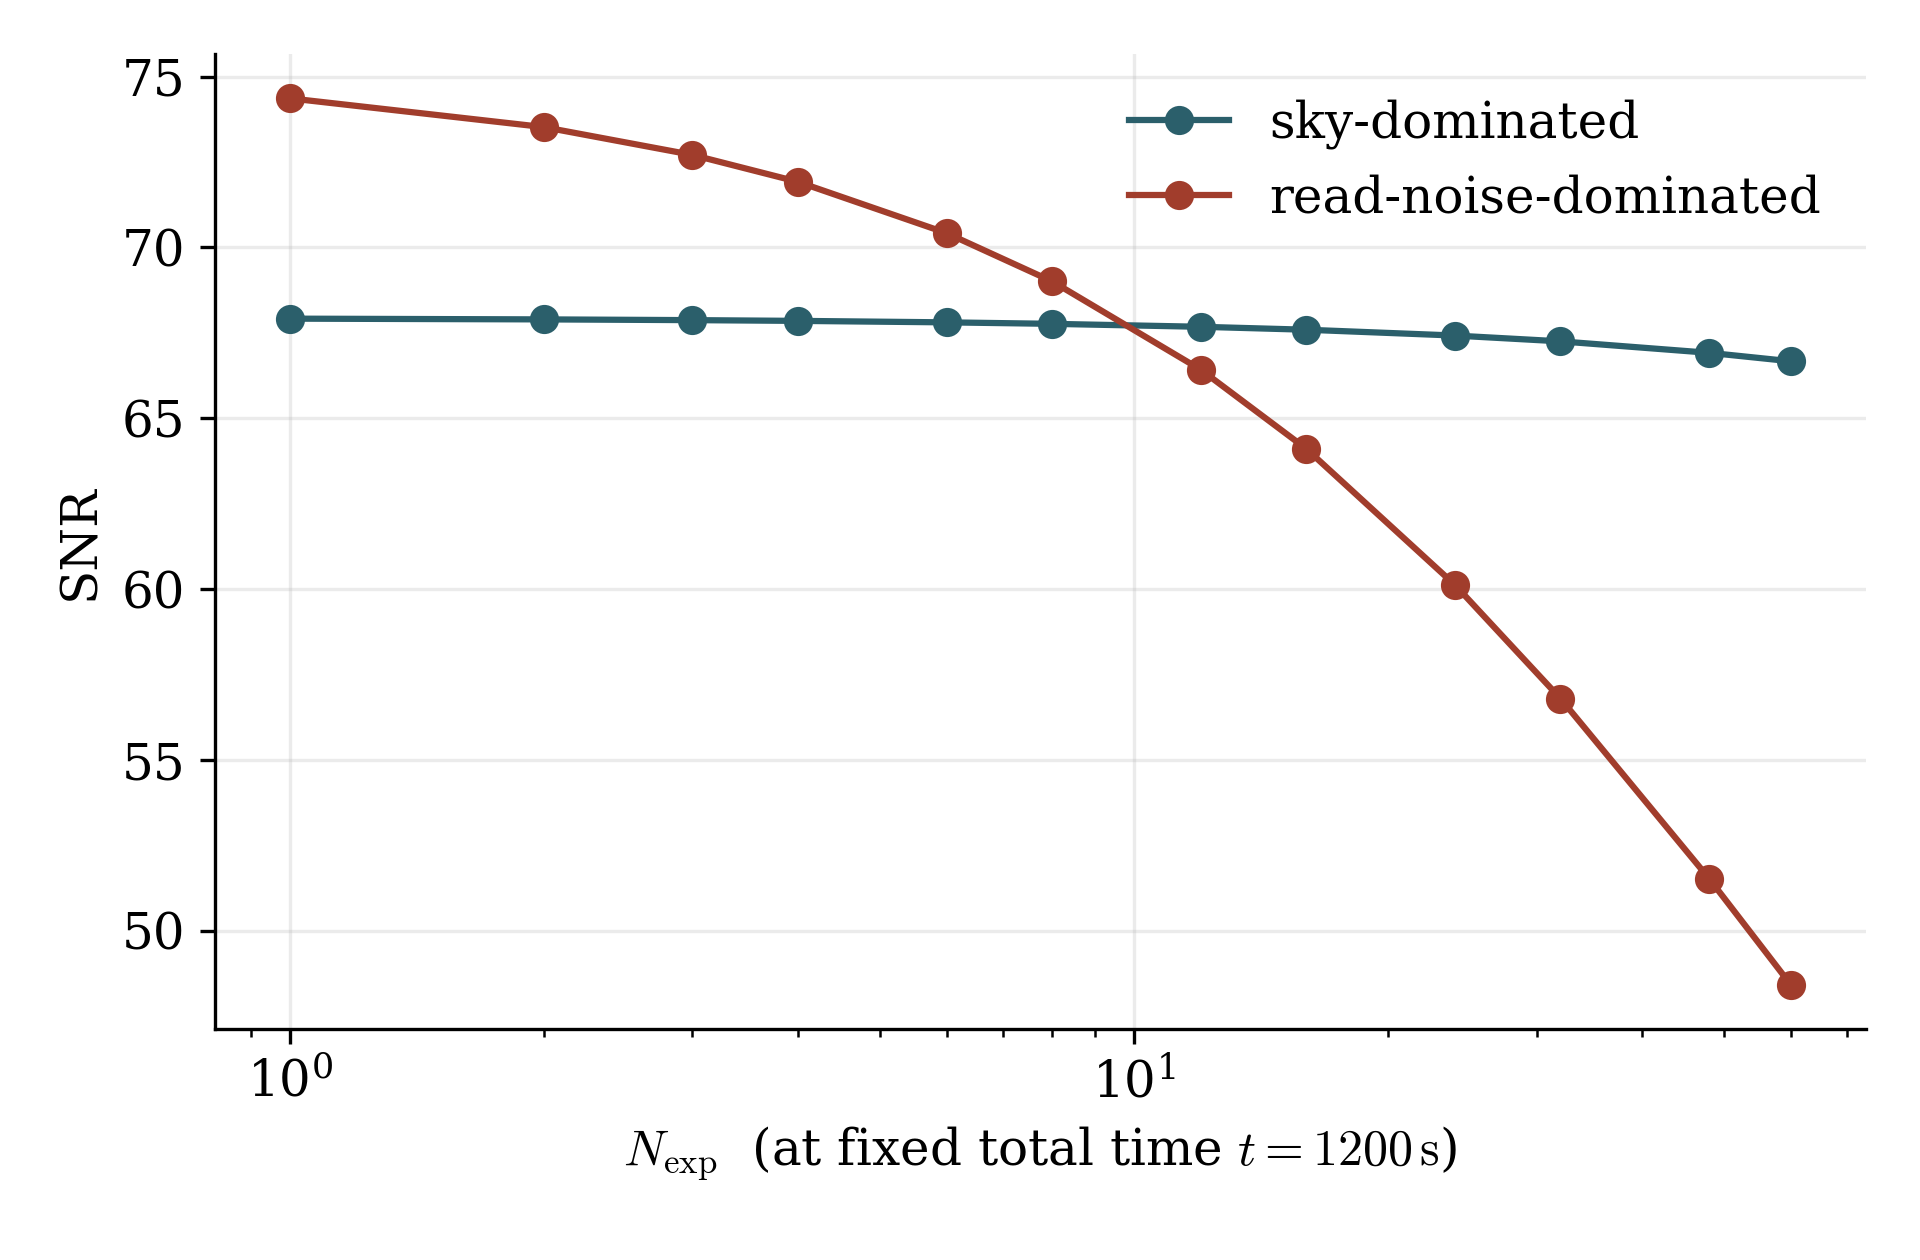
\includegraphics[width=0.85\textwidth]{figs/fig2_nexp.png}
		\caption{Signal-to-noise ratio as a function of the number of sub-exposures $N_{\rm exp}$ at fixed total exposure time $t = 1200\,\mathrm{s}$. In the sky-limited regime, the curve is virtually flat, making exposure splitting cost-free. In the read-noise-limited regime, each additional readout adds an unrecoverable noise penalty, degrading $\mathrm{SNR}$.}
		\label{fig:nexp_comparison}
	\end{figure}

	\section{Summary and Observational Decision Matrix}

	All photometric noise trade-offs are governed by which term in the variance sum $\sigma_{\rm tot}^2$ dominates. Table~\ref{tab:regime_summary} provides an operational decision matrix for planning astronomical exposures.

	\begin{table}[htbp]
		\centering
		\begin{tabular}{@{}l l l p{6.2cm}@{}}
			\toprule
			\textbf{Regime} & \textbf{Dominant Variance} & \textbf{SNR Scaling} & \textbf{Operational Strategy} \\
			\midrule
			Bright Source & $\sigma_{\rm src}^2 = R_{\rm src}t$ & $\mathrm{SNR} \propto \sqrt{t}$ & Monitor full-well capacity; prevent saturation and non-linearity. \\
			\addlinespace[0.4em]
			Sky-Limited & $\sigma_{\rm sky}^2 = n_{\rm pix}R_{\rm sky}t$ & $\mathrm{SNR} \propto \dfrac{\sqrt{t}}{\sqrt{n_{\rm pix}}}$ & Minimize aperture (exploit good seeing); freely split into $N_{\rm exp}$ sub-exposures for CR rejection. \\
			\addlinespace[0.4em]
			Read-Noise Limited & $\sigma_{\rm read}^2 = n_{\rm pix}N_{\rm exp}\sigma_{\rm RON}^2$ & $\mathrm{SNR} \propto \dfrac{1}{\sqrt{n_{\rm pix}N_{\rm exp}}}$ & Bin pixels on-chip (up to Nyquist sampling); maximize $t_{\rm exp}$ (minimize $N_{\rm exp}$) within CR limits. \\
			\bottomrule
		\end{tabular}
		\caption{Comparative overview of the three observational regimes, dominant noise terms, signal-to-noise scalings, and observing strategies.}
		\label{tab:regime_summary}
	\end{table}

	\FloatBarrier

\end{document}
